\documentclass[Harvard,Times1COL]{WileyNJDv5}


\usepackage{natbib}
\bibliographystyle{wileyNJD-Harvard}

\hypersetup{
  colorlinks=true,
  linkcolor=blue,
  citecolor=blue,
  filecolor=black,
  urlcolor=black
}
\begin{document}

\articletype{Article Type: Research Article}

\received{Date Month Year}
\revised{Date Month Year}
\accepted{Date Month Year}
\journal{Journal of Policy Analysis and Management}
\volume{00}
\copyyear{2025}
\startpage{1}

% TODO: Inherited from WileyNJD example. Is this needed?
% \raggedbottom


\authormark{Dupré and Morgenroth}

\presentaddress{DCU Business School, Dublin 9, Ireland.}



% Include information for each author
  \author[1]{Damien Dupré}
  \author[1]{Edgar Morgenroth}

% Include information for each affiliation
\address[1]{%
  \orgdiv{%
    Business School%
    , %
    \orgname{%
      Dublin City University%
      , %
    }%
    \orgaddress{%
      \state{Dublin}%
      , %
      \country{Ireland}%
    }%
  }%
}

% Include information for each corresponder
      \corres{%
      %
        Damien Dupré%
      %
      \email{damien.dupre@dcu.ie}%
    }
    
\title{Divergent Impacts of COVID-19 School Closures on Youth Infection
Dynamics: Evidence from 12 European Countries}
\titlemark{COVID-19 School Closures and Youth Infection Dynamics}

\abstract[Abstract]{The effectiveness of school closures as a COVID-19
control measure remains a subject of debate. This paper critically
reassesses their impact by examining infection trends across various age
groups in 12 European countries. We apply a dual analytical approach:
Generalised Additive Models (GAMs) are used to capture complex,
non-linear effects of closures on age-specific case numbers, while
Transfer Entropy (TE) is employed to quantify directional transmission
patterns between these age groups. Our findings reveal deviations from
commonly held assumptions. While school closures were associated with a
non-linear decline in overall national COVID-19 cases, the effects on
children and young adults varied considerably. A consistent downward
trend in infections was seen only in the pre-school age group. In
contrast, school-aged children experienced a marked rise in COVID-19
cases following an initial period of stability or slight decrease after
closures began. The Transfer Entropy analysis also identified
asymmetric, directional patterns in transmission, revealing that
infection trends in specific age groups could predict subsequent changes
in others. These results challenge the assumption that school closures
uniformly benefit younger populations and emphasise the need for
age-specific analysis in pandemic planning and support the development
of more nuanced, evidence-based public health policies.}

{\keywords{COVID-19, School closures, Intergenerational
transmission, Non-linear effects, Infection dynamics.}

\maketitle
\section{Introduction}\label{introduction}

The COVID-19 pandemic has had a profound impact on global health, with
an estimate of 14.83 million excess deaths globally
\citep{msemburi2023estimates}. Beyond direct mortality, the pandemic has
caused significant collateral damage, including losses of lives and
livelihoods, necessitating a comprehensive approach to measuring its
broader impacts. A wide range of non-pharmaceutical interventions (NPI)
were enacted to control the spread of COVID-19, especially before the
availability of effective vaccines. Due to their social mixing patterns,
children have been identified as an age group that can drive the spread
of respiratory infections such as influenza \citep{moser2018estimating},
and school closures were found to be effective in mitigating the spread
of influenza H1N1 in Japan in 2009 \citep{kawano2015substantial}. It is
therefore not surprising that school closures were one of the NPIs that
were introduced in many countries to stop the spread of COVID-19. They
were used particularly during the initial wave of the pandemic and
during subsequent waves when case numbers were high.

Recently, a body of literature has shown various negative consequences
on child development and health due to school closures. School closures
have been found to have negatively affected child mental health
\citep{moulin2022longitudinal}, nutrition/obesity
\citep{sugimoto2023temporal}, and education
\citep{lerkkanen2023reading}. Some governments were questioning their
decisions to close schools \citep{de2021determines}. For example, the
German health minister Karl Lauterbach, in an interview with one of
Germany's publicly funded television stations, admitted that ``in
retrospect it had been wrong to keep schools and childcare closed for so
long'' \citep{ard2023lauterbach}. Even if school closures had negative
consequences for children, they might nevertheless have been effective
at stopping the spread of COVID-19. However, analysis on the
effectiveness of school closures on the spread of COVID-19 remains
inconclusive. In a study of a panel of European countries,
\citet{alfano2022effects} found that school closures were associated
with a reduced COVID-19 incidence. In contrast, \citet{walsh2021school}
in a review of 40 studies covering 150 countries concluded that the
effectiveness of school closures was uncertain, with 60\% having
identified no impact and pointing to the potential for the analysis to
be affected by confounding factors and collinearity. The latter
shortcomings suggest that it is hard to draw firm inferences, as even a
positive result may not imply causality.

Once it was clear that COVID-19 spreads from person to person, it was
natural that governments were advised to enact measures to reduce social
contact in order to reduce the spread of the virus. Therefore, it is
legitimate to believe that by closing schools, a reduction of the
contaminations would be observed in the younger age groups. However, the
efficiency of school closure on the reduction of COVID-19 cases is still
questioned \citep{bayham2020impact, esposito2021comprehensive}. While
some research has found that school closures contribute to limit or to
reduce the growth rate of confirmed cases after implementation
\citep{stage2021shut, yoshiyuki2020effects}, others did not observe a
change in the evolution of COVID-19 cases
\citep{chang2020modelling, iwata2020school}. For instance, a controlled
comparison between similar localities in Japan with schools closed and
schools open did not reveal any evidence that school closures reduced
the spread of COVID-19 \citep{fukumoto2021no}. If the school closure had
a real impact on the evolution of confirmed COVID-19 cases, it should be
possible to observe a decrease or at least an inflection in the trend of
its evolution among younger age groups.

A second implicit belief regarding the effect of school closure on the
spread of COVID-19 is that school not only influences the spread of the
virus among children and teenagers but also has a knock-on effect on the
spread of the virus in older age groups, also called Secondary Attack
Rate (SAR). The contaminated children and teenagers would bring the
virus back home and would pass the virus on to their parents and
relatives. For example, research investigating the contamination in the
household network not only revealed an exceptionally high rate of
secondary contamination but also that this contamination happened when
the schools were closed \citep{sorianoarandes2021household}. Despite
being reported in several clinical and epidemiological studies
\citep{siebach2021childhood, zhendong2020clinical}, multiple research
have shown that the SAR from children to household members was lower
than expected
\citep{heavey2020evidence, vanderhoek2020role, kim2021role, ludvigsson2020children}.
However, the SAR of children and teenagers to the household member is
likely to be age-dependent, with differences between infants, primary
and secondary school children, and college students
\citep{grasleguen2021reopening}. If a secondary transmission from
children and teenagers to household member has a significant influence,
then a temporal causality relationship between their evolution should be
observed.

A gap in these previous analyses is the insufficient granularity in
examining age-specific effects and the complex dynamics of inter-age
group transmission. This study aims to address these deficiencies by
providing a more robust and nuanced assessment. First, Generalized
Additive Models (GAMs) are utilized to flexibly model and quantify the
potentially non-linear evolution of COVID-19 cases following school
closures, specifically within these fine-grained age brackets. This
allows us to move beyond simple pre-post comparisons and capture dynamic
temporal patterns. Then, Transfer Entropy (TE), an information-theoretic
measure, is applied to assess directional causality in time series data.
TE is particularly adept at identifying how past states of one variable
(e.g., cases in one age group) influence future states of another (e.g.,
cases in a different age group), even in complex, non-linear systems
like epidemic spread. This dual methodology allows for a deeper
understanding of both the direct age-specific consequences of school
closures and the potential for altered intergenerational transmission
dynamics. Our findings challenge simplistic narratives about school
closure efficacy and highlight the importance of age-stratified analysis
for future pandemic preparedness.

\section{Methods}\label{methods}

\subsection{Study design}\label{study-design}

A longitudinal study was conducted to observe changes in COVID-19 cases
during school closures. Changes in COVID-19 from five age groups from
the first to the 28th day of school closure are compared across 12
countries. Then, a causality analysis evaluate the impact of changes in
these younger groups on older age groups.

\subsection{Data collection}\label{data-collection}

Data on COVID-19 case counts by age group have been obtained from the
COVerAGE-DB project \citep{riffe2021data}. The COVerAGE-DB which collect
numbers for every countries by groups of 5 or 10 years if available. In
addition, spline approximations are used to deals with the heterogeneity
of countries' reporting formats by using when the data for this age
bracket is not available for a country. Countries communicating data
with groups of 5 years were chosen to match as much as possible the
different school stages.

To identify the impact of school closures on the number of cases,
information regarding the school closures on a day-by-day basis is
required, and this is taken from the ``UNESCO global education
coalition'' (2022). For each day, in each country, the status of the
schools is indicated as fully open, partially open, closed due to
COVID-19, or closed due to an academic break. Because it would be
difficult to measure the effect of school closures at a country level
when schools are partially closed, only closures due to COVID-19 or due
to an academic break are considered. Indeed, both are considered as
closure at a country-wide level. Any COVID-19 case numbers beyond the
28-day period are not relevant for evaluating the impact of school
closures.

\subsection{Data validation}\label{data-validation}

In order to cross-validate the data obtained after spline
approximations, a comparison with the data published by the
\citet{who2022https} reveals perfect similarities. The original data
consist of 14,089,320 observations of 10 variables (117 distinct
countries, region within the country, a unique observation code, the
date of the observation, the gender, which can be male, female, or both,
the age bracket by 5 years from 0 to 100, a confirmation of the age
interval for each bracket, the total number of cases so far, the total
number of deaths, and the total number of tests performed) from February
16, 2020 to January 20, 2022. After removing countries with missing and
inconsistent values, only 22 are suitable for data analyses. However, to
focus this analysis on geographically and culturally comparable
countries, only 12 European countries are kept: Austria, Belgium,
Bulgaria, Croatia, Estonia, France, Germany, Greece, Netherlands,
Portugal, Slovakia, and Spain. The observations are reported in terms of
the total number of COVID-19 cases per day from the start of the
pandemic. The daily number of cases at a specific date \(n\prime_{t}\)
is calculated with the difference between the total cases at a date
\(t\) and the total cases at a date \(t-1\) (i.e., derivative 1). In
addition, the change in the daily number of cases \(n\prime\prime_{t}\)
between \(n\prime_{t}\) and \(n\prime_{t-1}\) has also been calculated
(i.e., derivative 2).

\subsection{Controlling for confounding Non-Pharmaceutical
Interventions}\label{controlling-for-confounding-non-pharmaceutical-interventions}

Recognizing that school closures rarely occurred in isolation, a
critical component of this analysis was to account for other
contemporaneous NPIs. To mitigate confounding from other NPIs, we
incorporated four time-varying composite NPI index identified by the
Oxford COVID-19 Government Response Tracker (OxCGRT) project
\citep{hale2021global}: the average stringency index, the average
government response index, the average containment health index, and the
average economic support index. Specific data were collected from each
country on various policy responses governments implemented to curb the
spread of COVID-19, such as travel restrictions, workplace closures,
public event cancellations, restrictions on gatherings, or public health
messaging. These indicators were then aggregated to create indexes,
reflecting the overall level of government restrictions.

\subsection{Generalized additive
model}\label{generalized-additive-model}

The effect of school closure on the trend of daily COVID-19 cases is
analysed using a Generalized Additive Model (GAM). GAM is a flexible
modelling approach that estimates non-linear relationships between
variables. Compared to other methods such as Vector Autoregression, GAM
can handle fixed and random smooth effects without making strict
assumptions about linearity.

The GAM is fitted on the daily COVID-19 cases to test the hypothesis of
a significant non-linear evolution of cases among age groups from 0 to
4, from 5 to 9, from 10 to 14, from 15 to 19, and from 20 to 24
\citep{wood2017generalized}. The model also estimates the overall
non-linear effect by country, taking into account the interaction
between age groups and countries as random intercepts and the
interaction between time, countries, and the period of closure as random
effects (Eq \ref{eq-gam}).

By estimating the degree of smoothness of a Bayesian spline smoothing
using restricted fast maximum likelihood estimation
\citep{wood2011fast}, GAM identifies dynamic patterns underlying the
evolution of COVID-19 cases reported while including the random effect
of different age groups and countries as follows:

\begin{equation}\phantomsection\label{eq-gam}{
\begin{aligned}[t]
  n\prime_t &\sim \text{Poisson}(\lambda_t) \\
  \log(\lambda_t) &= \beta_0 + \beta_1\,wave_t + \beta_2\,country_t + \beta_3\,age\,group_t \\
  &\quad + f_1(closure_t) + f_2(closure_t, country_t) \\
  &\quad + f_3(closure_t, age\,group_t) + f_4(stringency\,index_t) \\
  &\quad + f_5(government\,response\,index_t) + f_6(containment\,health\,index_t) \\
  &\quad + f_7(economic\,support\,index_t) +\epsilon_t
\end{aligned}
}\end{equation}

\noindent where \(n\prime_t\) represents the confirmed COVID-19 cases,
assuming a Poisson distribution for the fitting \citep{loader2006local},
and \(t\) is the date corresponding to the confirmed COVID-19 cases. The
response variable includes a specific random effect taking into account
variation within waves of school closure, countries, and age groups. The
terms \(f_1\) to \(f_3\) are smooth functions of the time since closure,
the time since closure for each country, and the time since closure for
each age group. The terms \(f_4\) to \(f_7\) are random effects
corresponding to the average stringency index, the average government
response index, the average containment health index, and the average
economic support index. The restricted maximum likelihood (REML) was
used to avoid over fitting while estimating smoothing parameters. In
order to accurately account for the autocorrelation arising from the
time series data, the residuals are modelled using an AR1 error model
such as
\(\epsilon_t = \phi \epsilon_{t-1} + \eta_t, \quad \eta_t \sim \mathcal{N}(0, \sigma^2)\)
where \(\phi\) is the autoregressive parameter. By incorporating the
autoregressive component, the AR1 model acknowledges the dependence of
each residual on its previous value, thus providing a comprehensive
representation of the data's temporal dynamics.

Chi-square statistics were employed to assess if the degree of
smoothness is significantly different from zero.

\subsection{Transfer entropy}\label{transfer-entropy}

Transfer entropy (\(T\)) is a measure of the directional information
flow between two time series \(X\) and \(Y\), capturing how the past
values of one variable can predict changes in another. Unlike
correlation, transfer entropy accounts for the temporal order of events
and non-linear relationships, making it particularly suited for studying
dynamic systems such as epidemic data. In this analysis, transfer
entropy quantifies how case counts in one age group \(X\) influence
subsequent case counts in another age group \(Y\), providing insights
into directional transmission patterns. If it does, \(T\) is considered
evidence of a causal effect from the age group \(X\) to the age group
\(Y\) \citep{schreiber2000measuring}. As such, Granger causality is a
special case of transfer entropy applied to time series that are jointly
Gaussian distributed \citep{barnett2009granger}. Therefore, transfer
entropy is a more robust analysis of time series, especially when
applied to the impact of age cohorts on pandemic transmission
\citep{kissler2020symbolic}.

The influence of the evolution in COVID-19 cases across all age groups
is evaluated using Shannon's transfer entropy, given by:

\begin{equation}\phantomsection\label{eq-te}{
\begin{aligned}[t]
  T_{ag\,x \rightarrow ag\,y}(k,l) = \sum_{ag\,x_{t+1}, ag\,x_t^{(k)}, ag\,y_t^{(l)}} 
  p\left(ag\,x_{t+1}, ag\,x_t^{(k)}, ag\,y_t^{(l)}\right) 
  \log \left(\frac{p\left(ag\,x_{t+1} \mid ag\,x_t^{(k)}, ag\,y_t^{(l)}\right)}{p\left(ag\,x_{t+1} \mid ag\,x_t^{(k)}\right)}\right)
\end{aligned}
}\end{equation}

\noindent where \(T_{ag\,x \rightarrow\,ag\,y}\) consequently measures
the influence of the change dynamic from an age group \(X\) (or
\(ag\,x\)) to another age group \(Y\) (or \(ag\,y\)) for every country
(Eq \ref{eq-te}).

The day-by-day difference in COVID-19 confirmed cases
\(n\prime\prime_t\) is used to satisfy the stationary requirement for
the calculation of Shannon's Transfer Entropy
\citep{shannon1948mathematical, behrendt2019rtransferentropy}.

\section{Results}\label{results}

The data show that the trend of confirmed COVID-19 cases follows similar
patterns across the selected European countries, with scales following
the size of the population in these countries
(Figure~\ref{fig-overall}). Thus, the bigger the country, the higher the
total number of COVID-19 cases.

\begin{figure}[h]

\centering{

\pandocbounded{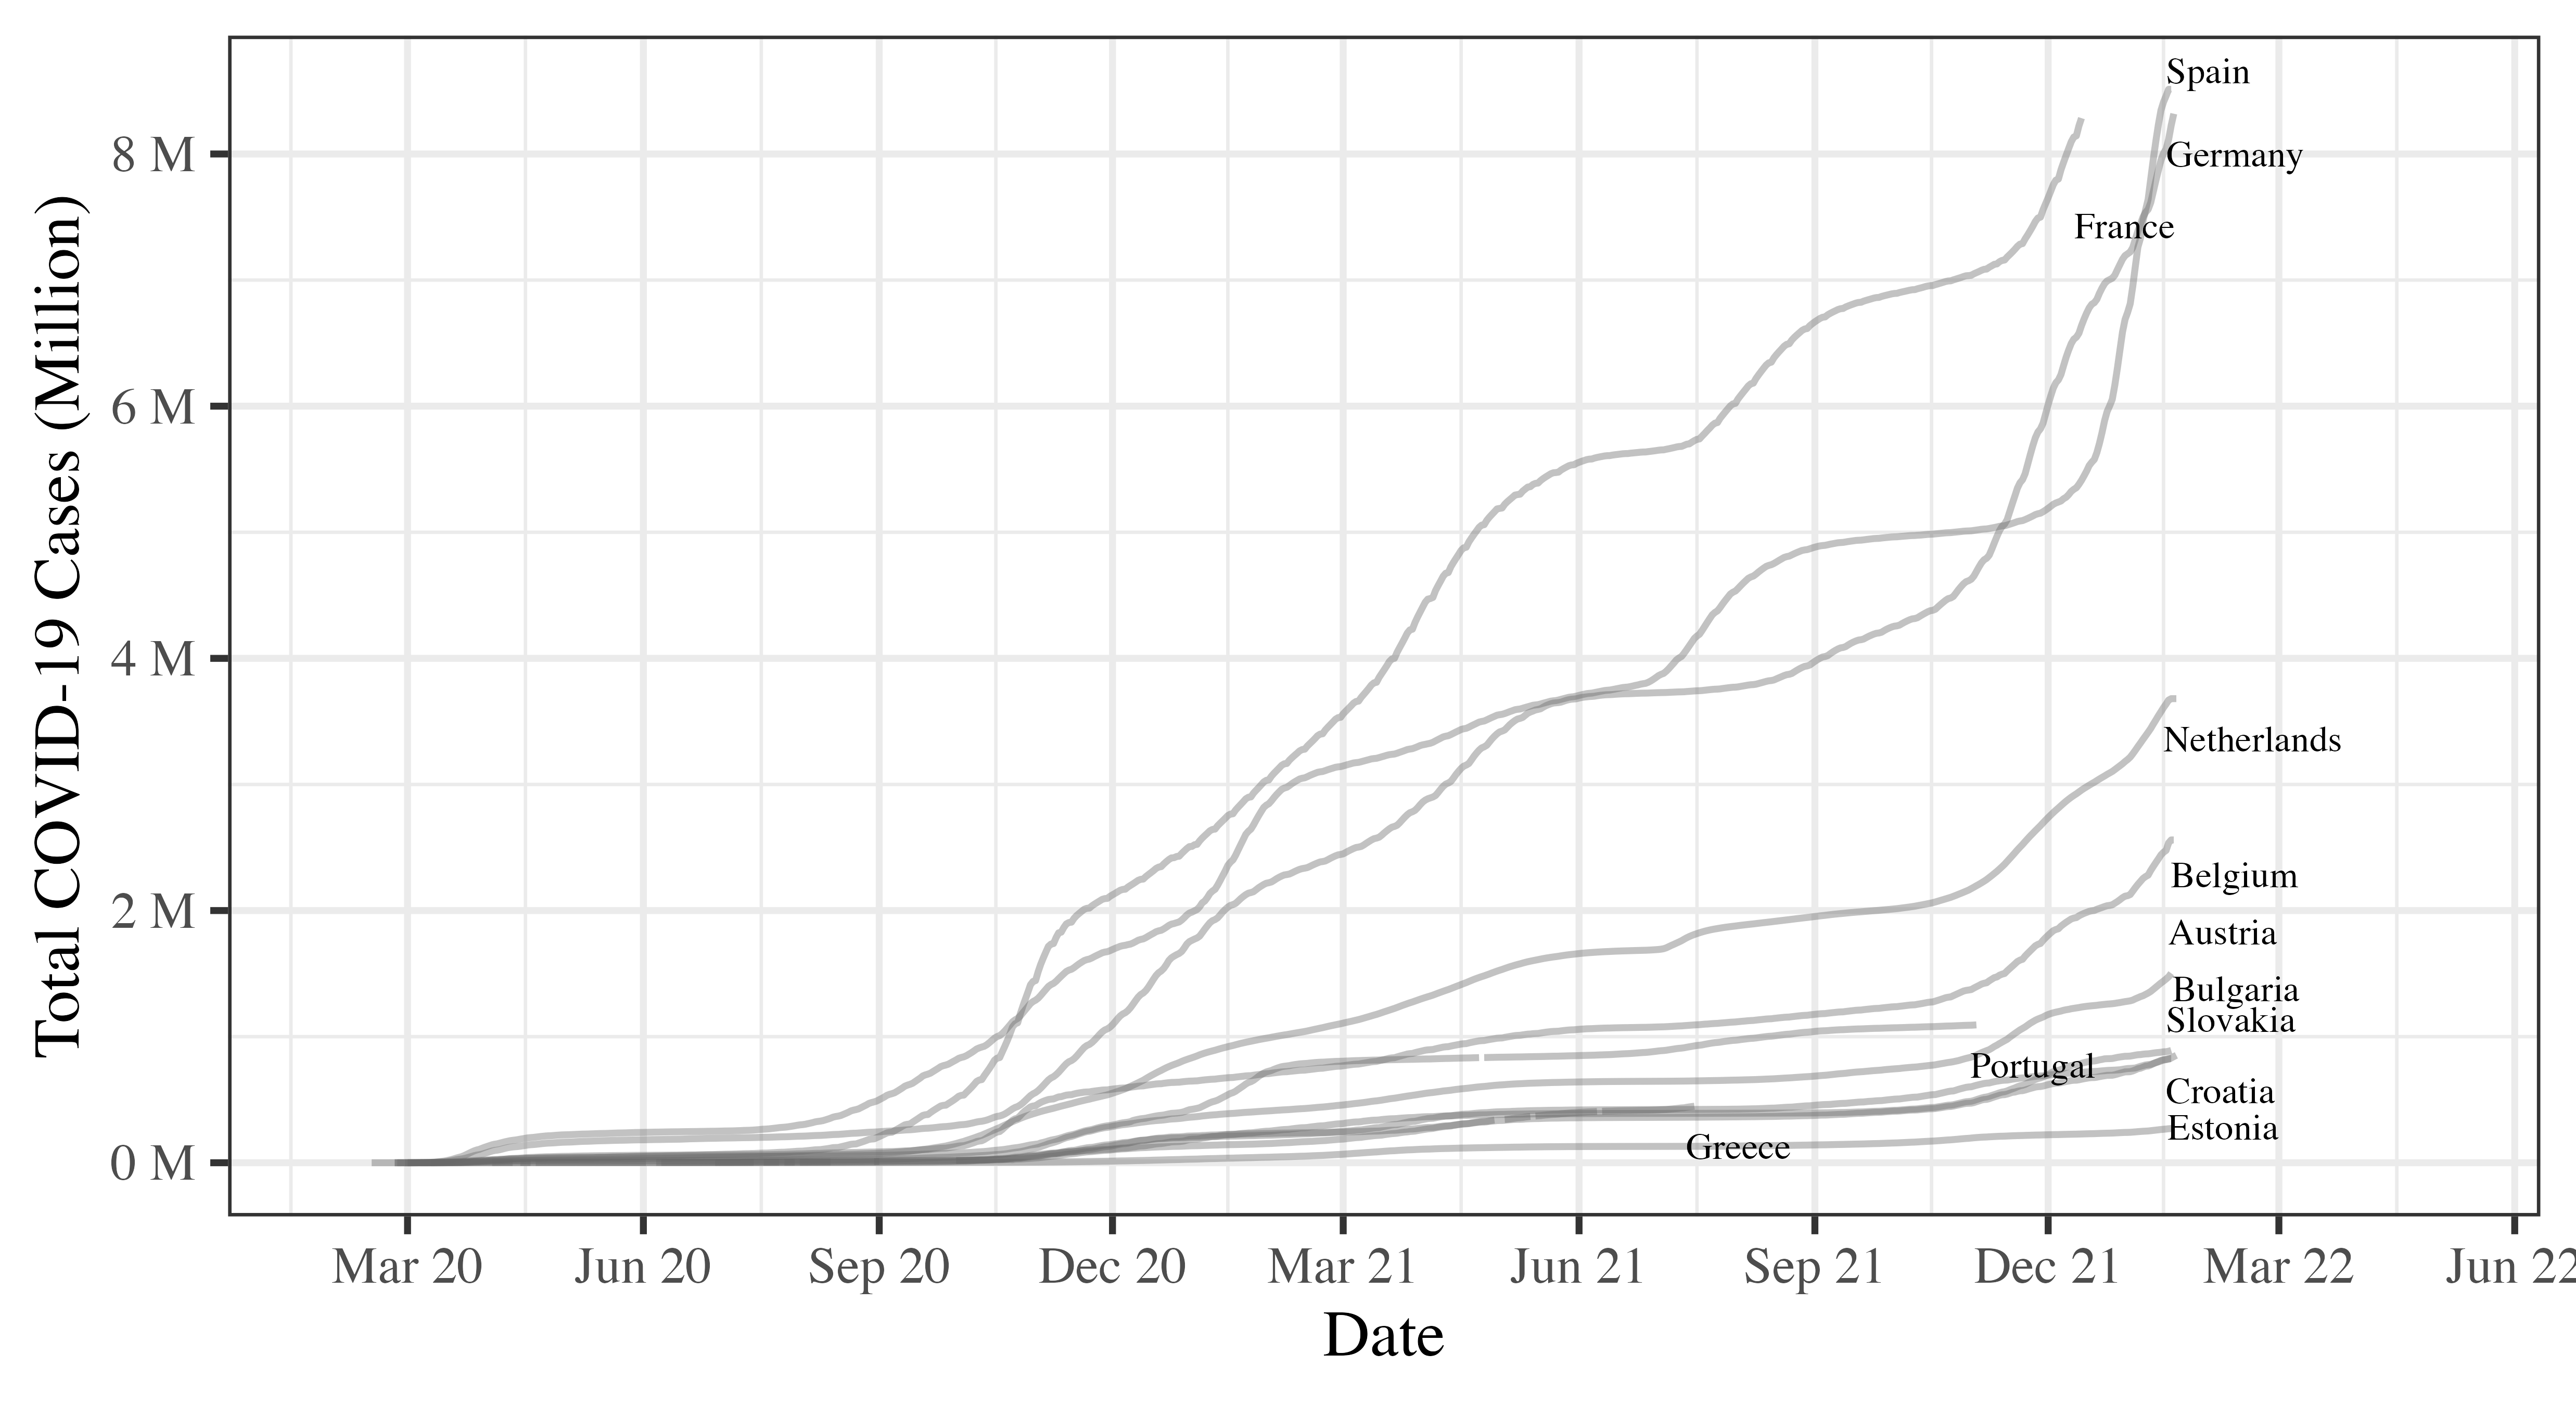
\includegraphics[keepaspectratio]{manuscript_files/figure-pdf/fig-overall-1.png}}

}

\caption{\label{fig-overall}Cumulative COVID-19 cases number for
selected European countries since the beginning of the pandemic. Source:
COVerAGE-DB \citep{riffe2021data}.}

\end{figure}%

The evolution of COVID-19 cases reveals some similarities across all age
groups. However, the influence of each wave on individual age groups
also has some particularities (Figure~\ref{fig-descriptive}). For
example, the first wave was more important among the oldest age groups,
whereas the third wave was more important among the youngest age groups.

\begin{figure}[h]

\centering{

\pandocbounded{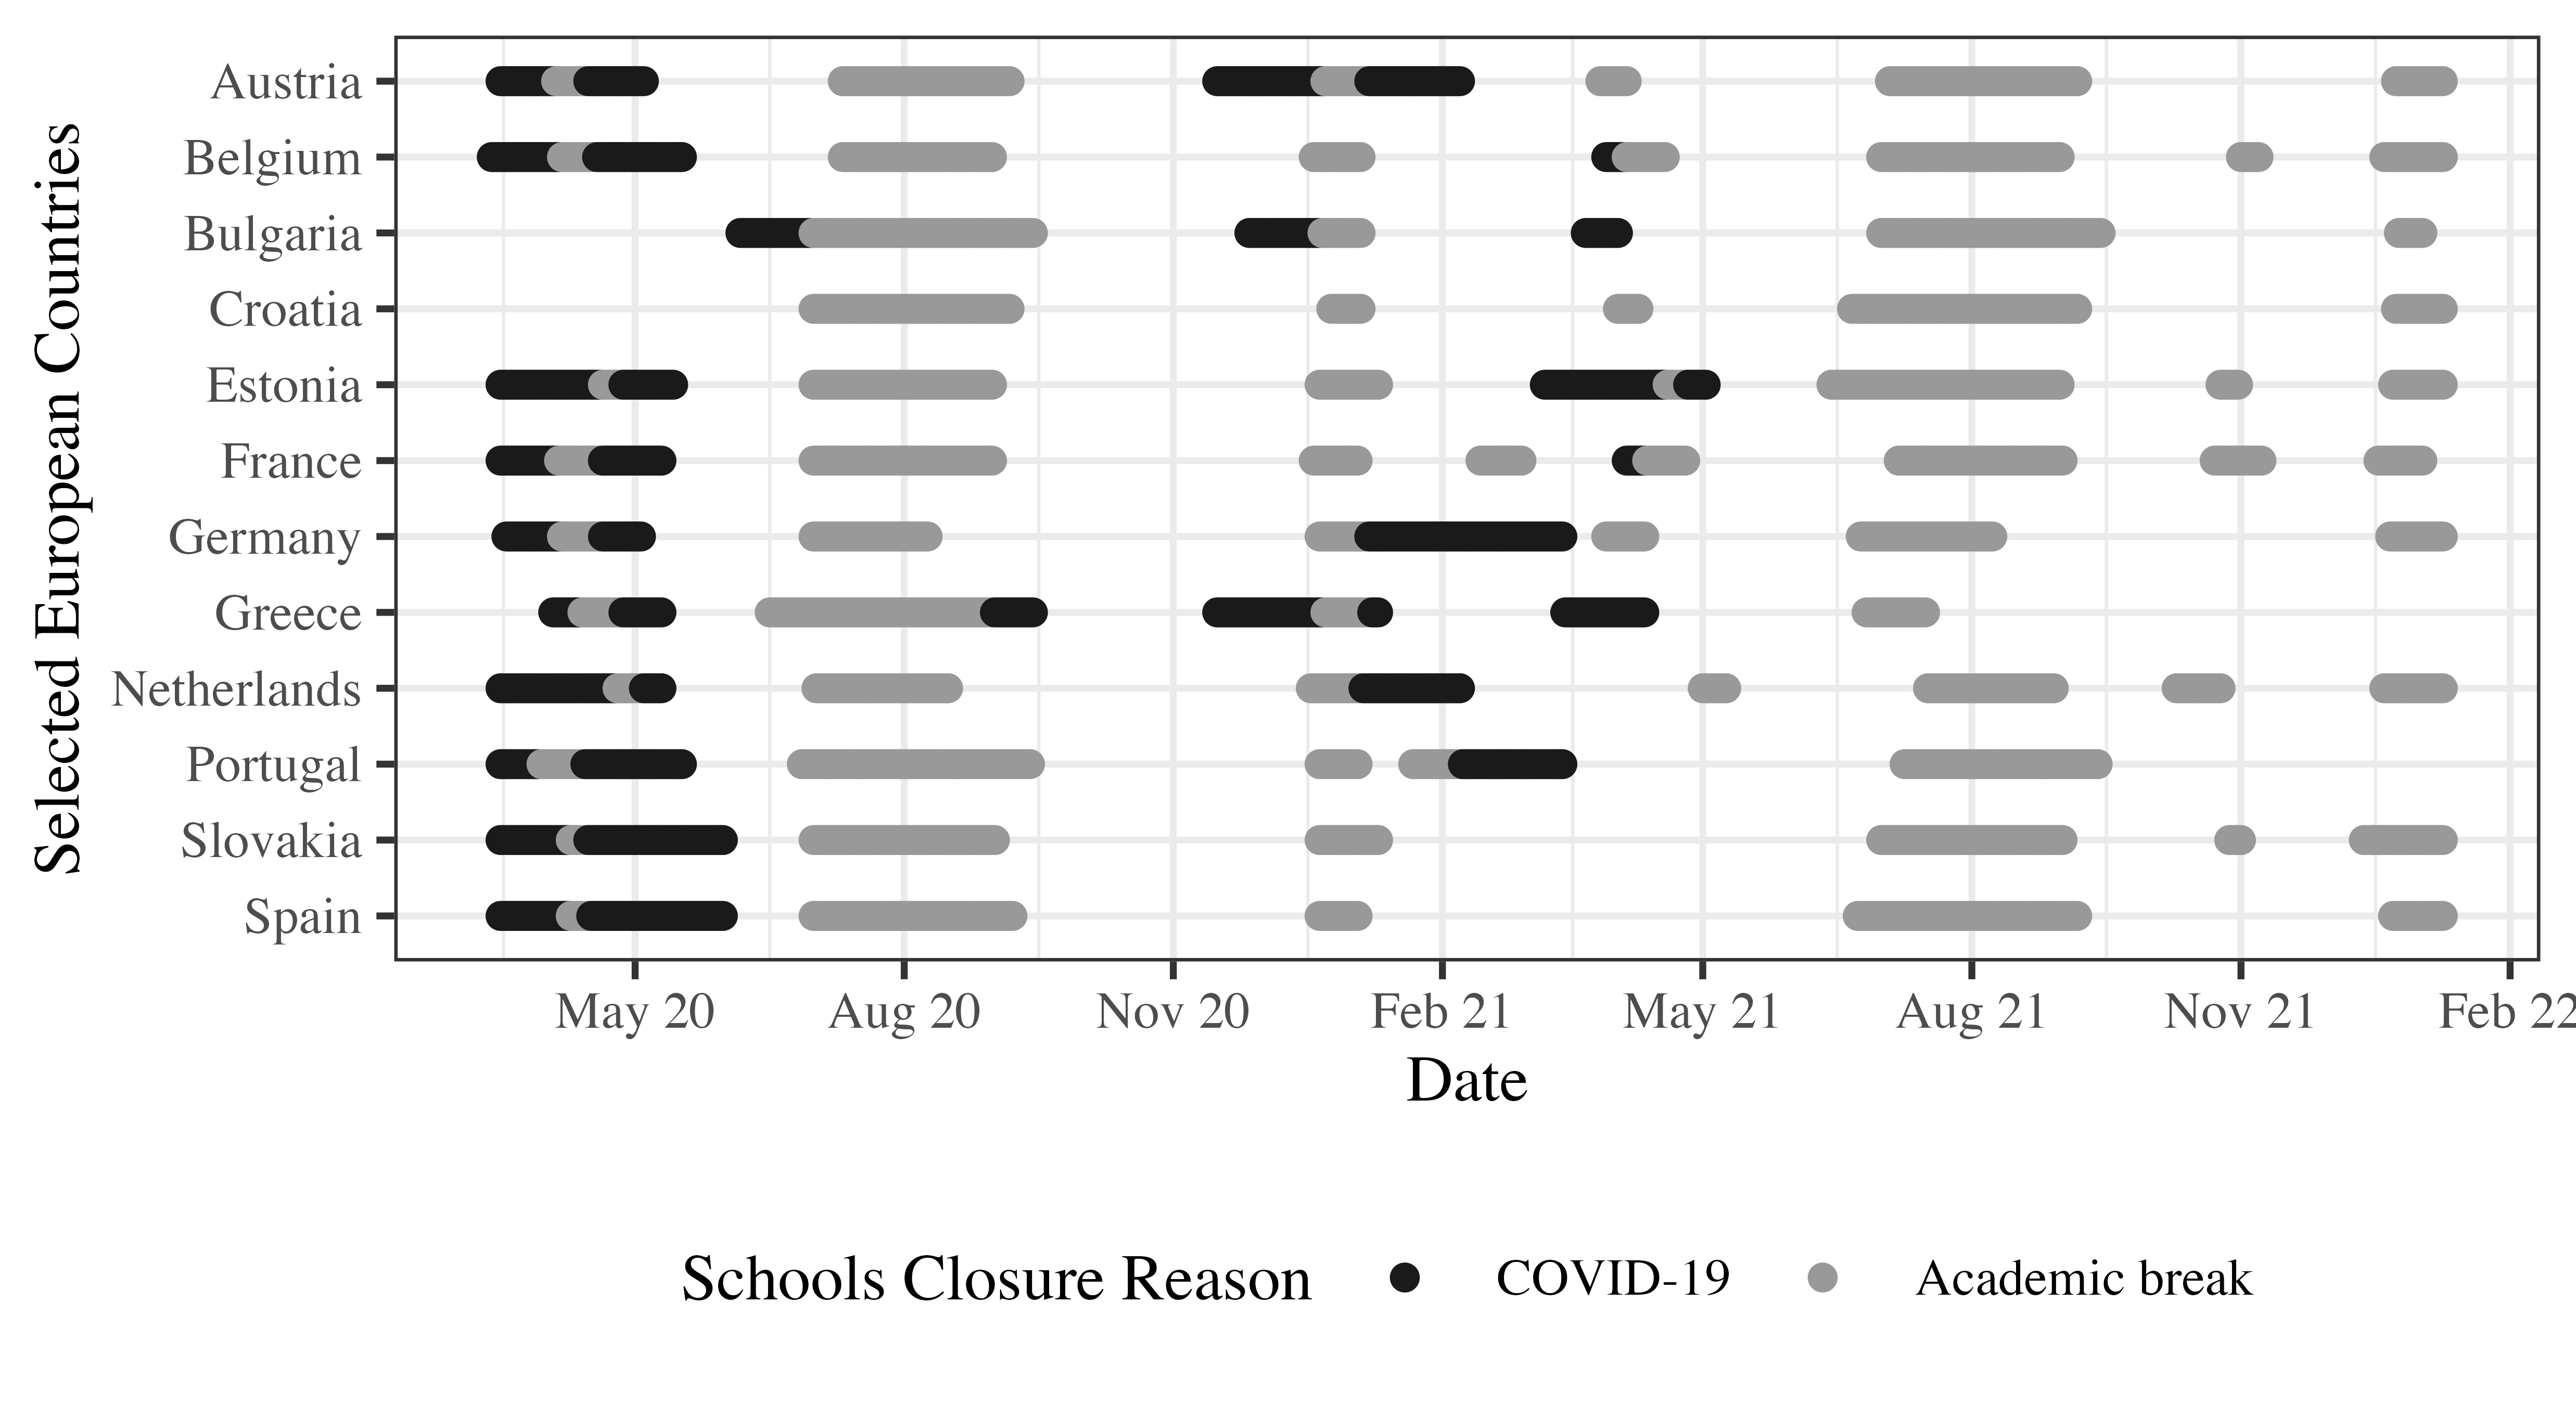
\includegraphics[keepaspectratio]{manuscript_files/figure-pdf/fig-descriptive-1.png}}

}

\caption{\label{fig-descriptive}Periods of school closure since the
beginning of the COVID-19 pandemic for selected European countries and
their reason: regular academic break versus closure due to government
decisions. Source: \citet{unesco2022https}.}

\end{figure}%

As outlined above, to evaluate the shape of the trend in the numbers of
COVID-19 cases reported after the three school closures longer than 21
consecutive days, a GAM was fitted as described above, taking into
account the overall effect across all the selected European countries,
as well as the effect for age groups: 0 to 4, 5 to 9, 10 to 14, 15 to
19, and 20 to 24 years old. The obtained results satisfy the
requirements to fit this model, which explains 80.2\% of the variation
in COVID-19 cases (Figure~\ref{fig-age}).

\begin{figure}[h]

\centering{

\pandocbounded{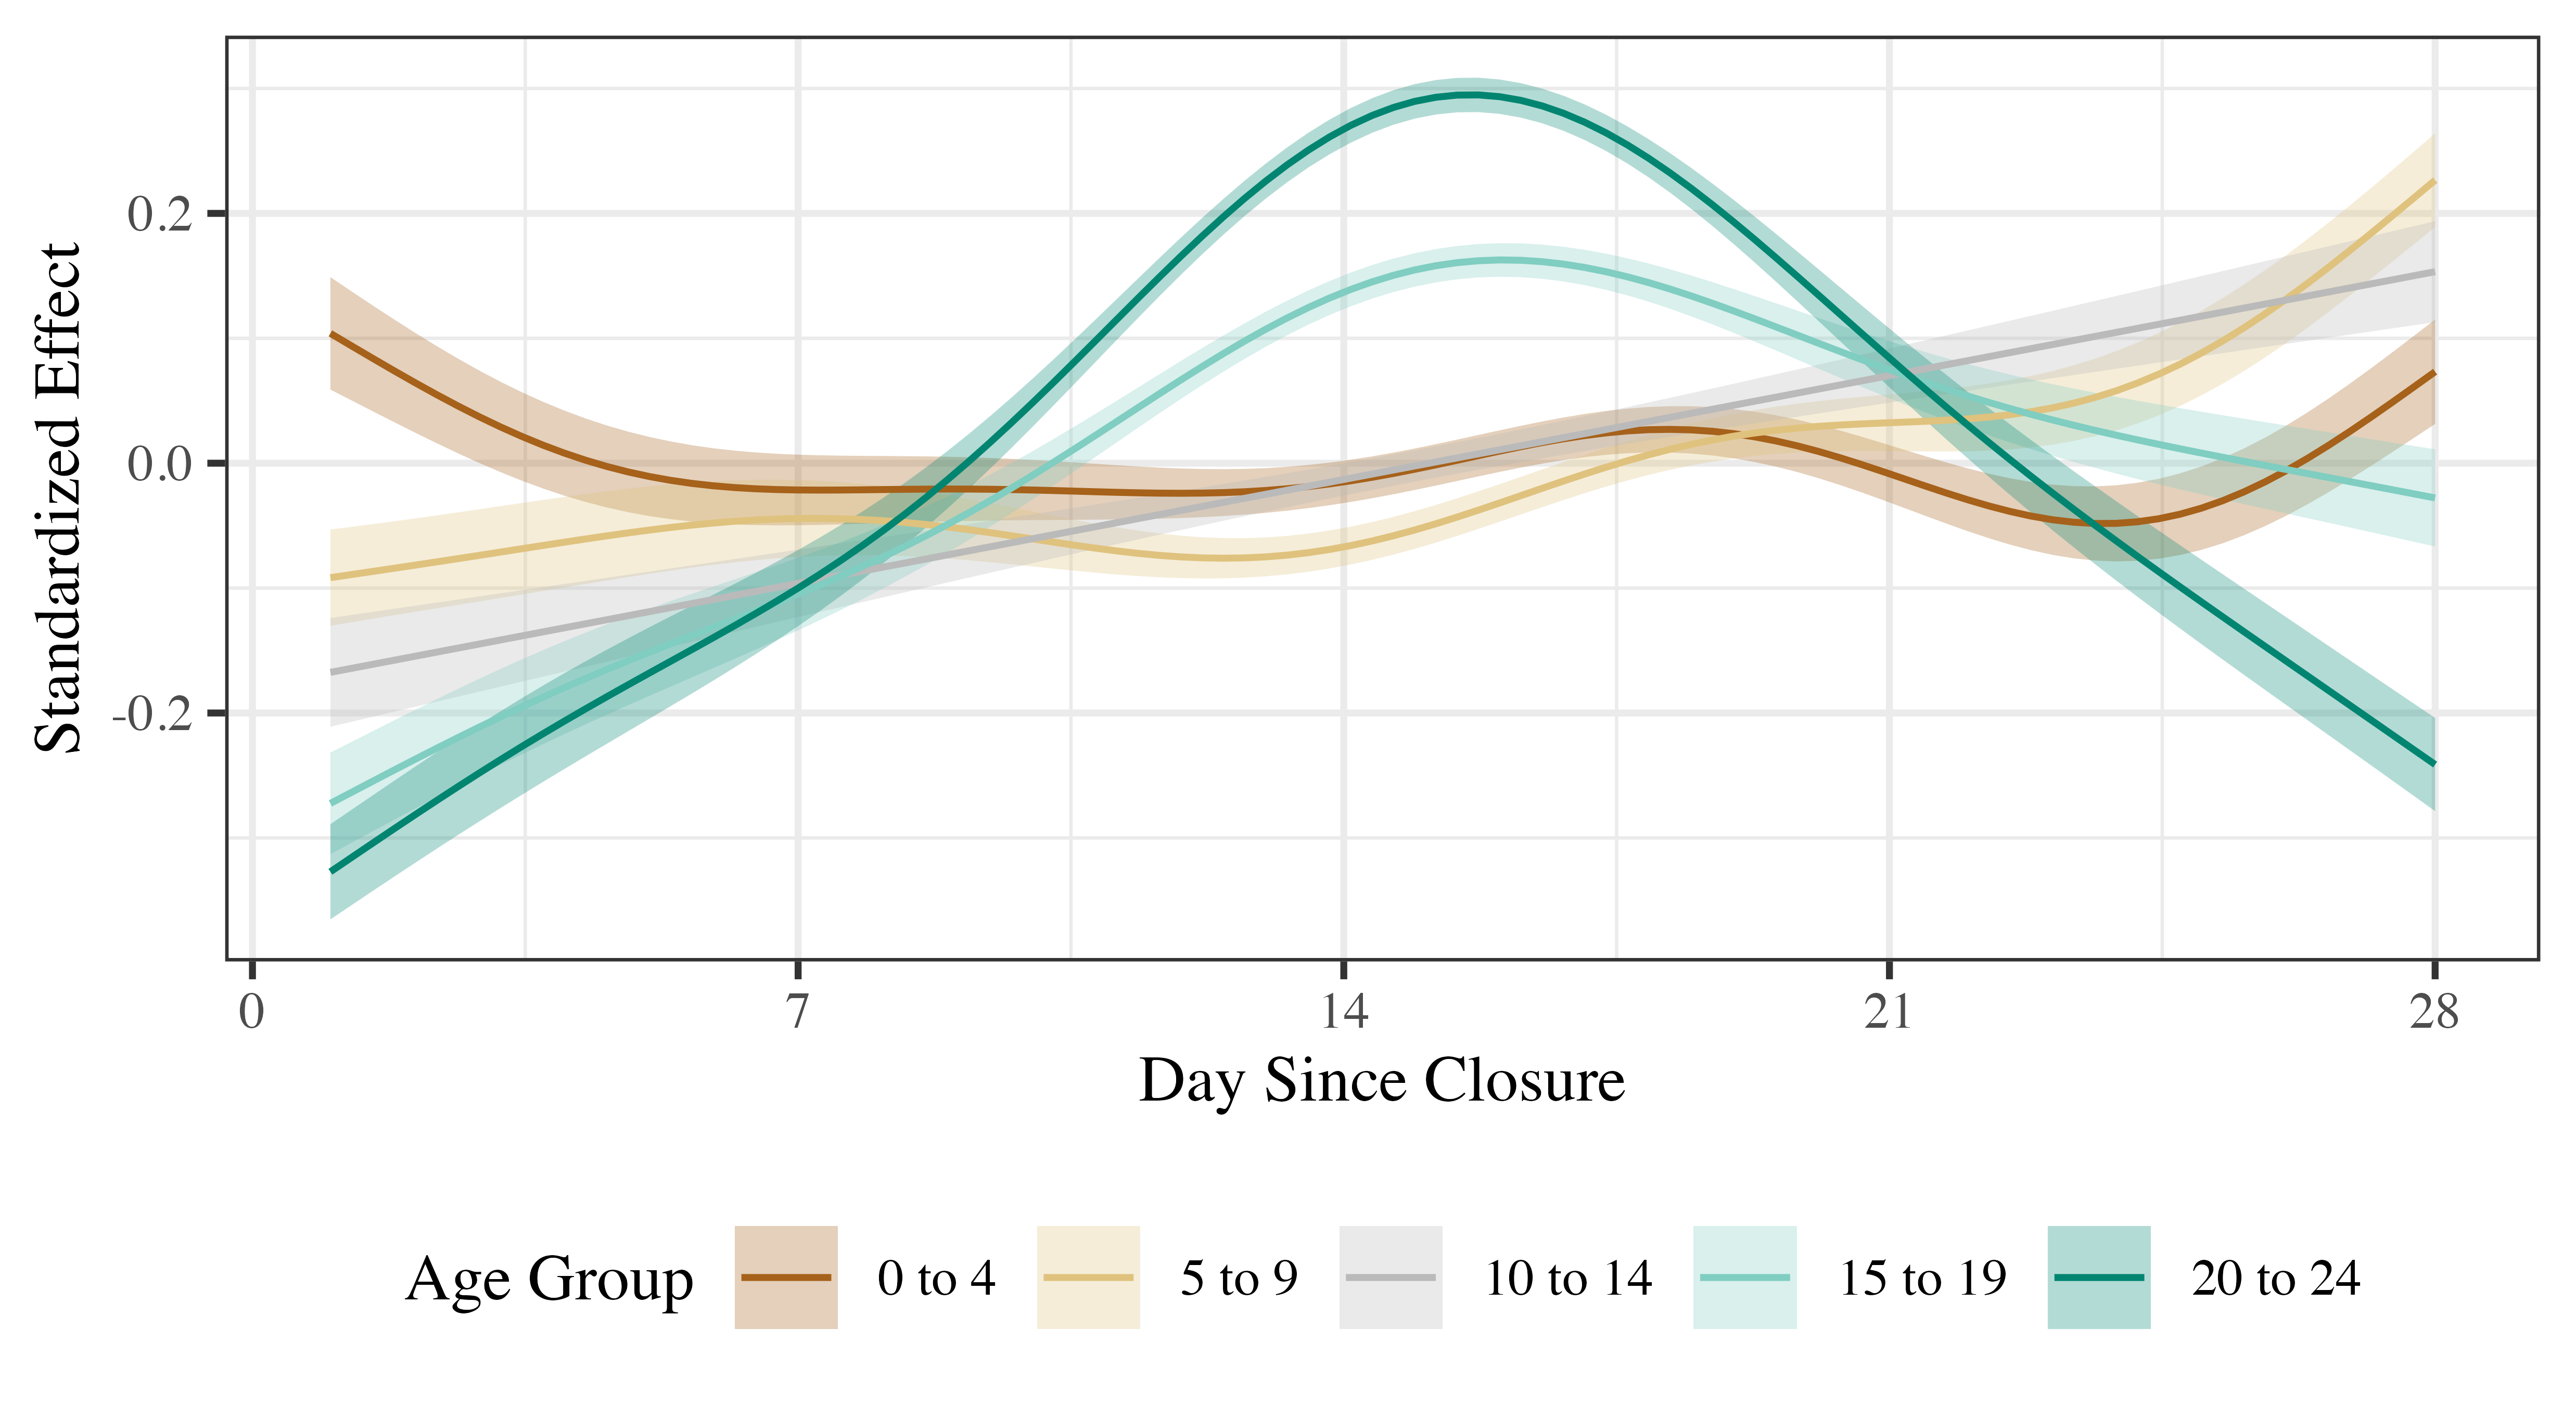
\includegraphics[keepaspectratio]{manuscript_files/figure-pdf/fig-age-1.png}}

}

\caption{\label{fig-age}Standardized effect of the smooth term in
Generalized Additive Model by age group. Standardized effects are
reported to compare the shape of the curve between age groups.}

\end{figure}%

Overall, the results revealed a decreasing non-linear effect of school
closure at a country level for the selected European countries (Austria:
\(\chi^2(5.82) = 3243.01\), \(p < 0.001\); Belgium:
\(\chi^2(5.98) = 6206.45\), \(p < 0.001\); Bulgaria:
\(\chi^2(5.89) = 258.19\), \(p < 0.001\); Croatia:
\(\chi^2(5.1) = 740.24\), \(p < 0.001\); Estonia:
\(\chi^2(5.93) = 1834.26\), \(p < 0.001\); France:
\(\chi^2(1) = 2412.59\), \(p < 0.001\); Germany
(\(\chi^2(5.98) = 3081.05\), \(p < 0.001\)); Greece:
\(\chi^2(5.95) = 2423.67\), \(p < 0.001\); The Netherlands:
\(\chi^2(4.97) = 5878.92\), \(p < 0.001\); Portugal:
\(\chi^2(5.94) = 2692.56\), \(p < 0.001\); Slovakia
(\(\chi^2(5.97) = 5335.74\), \(p < 0.001\); Spain:
\(\chi^2(5.94) = 498.09\), \(p < 0.001\), see Figure~\ref{fig-country}.

\begin{figure}[h]

\centering{

\pandocbounded{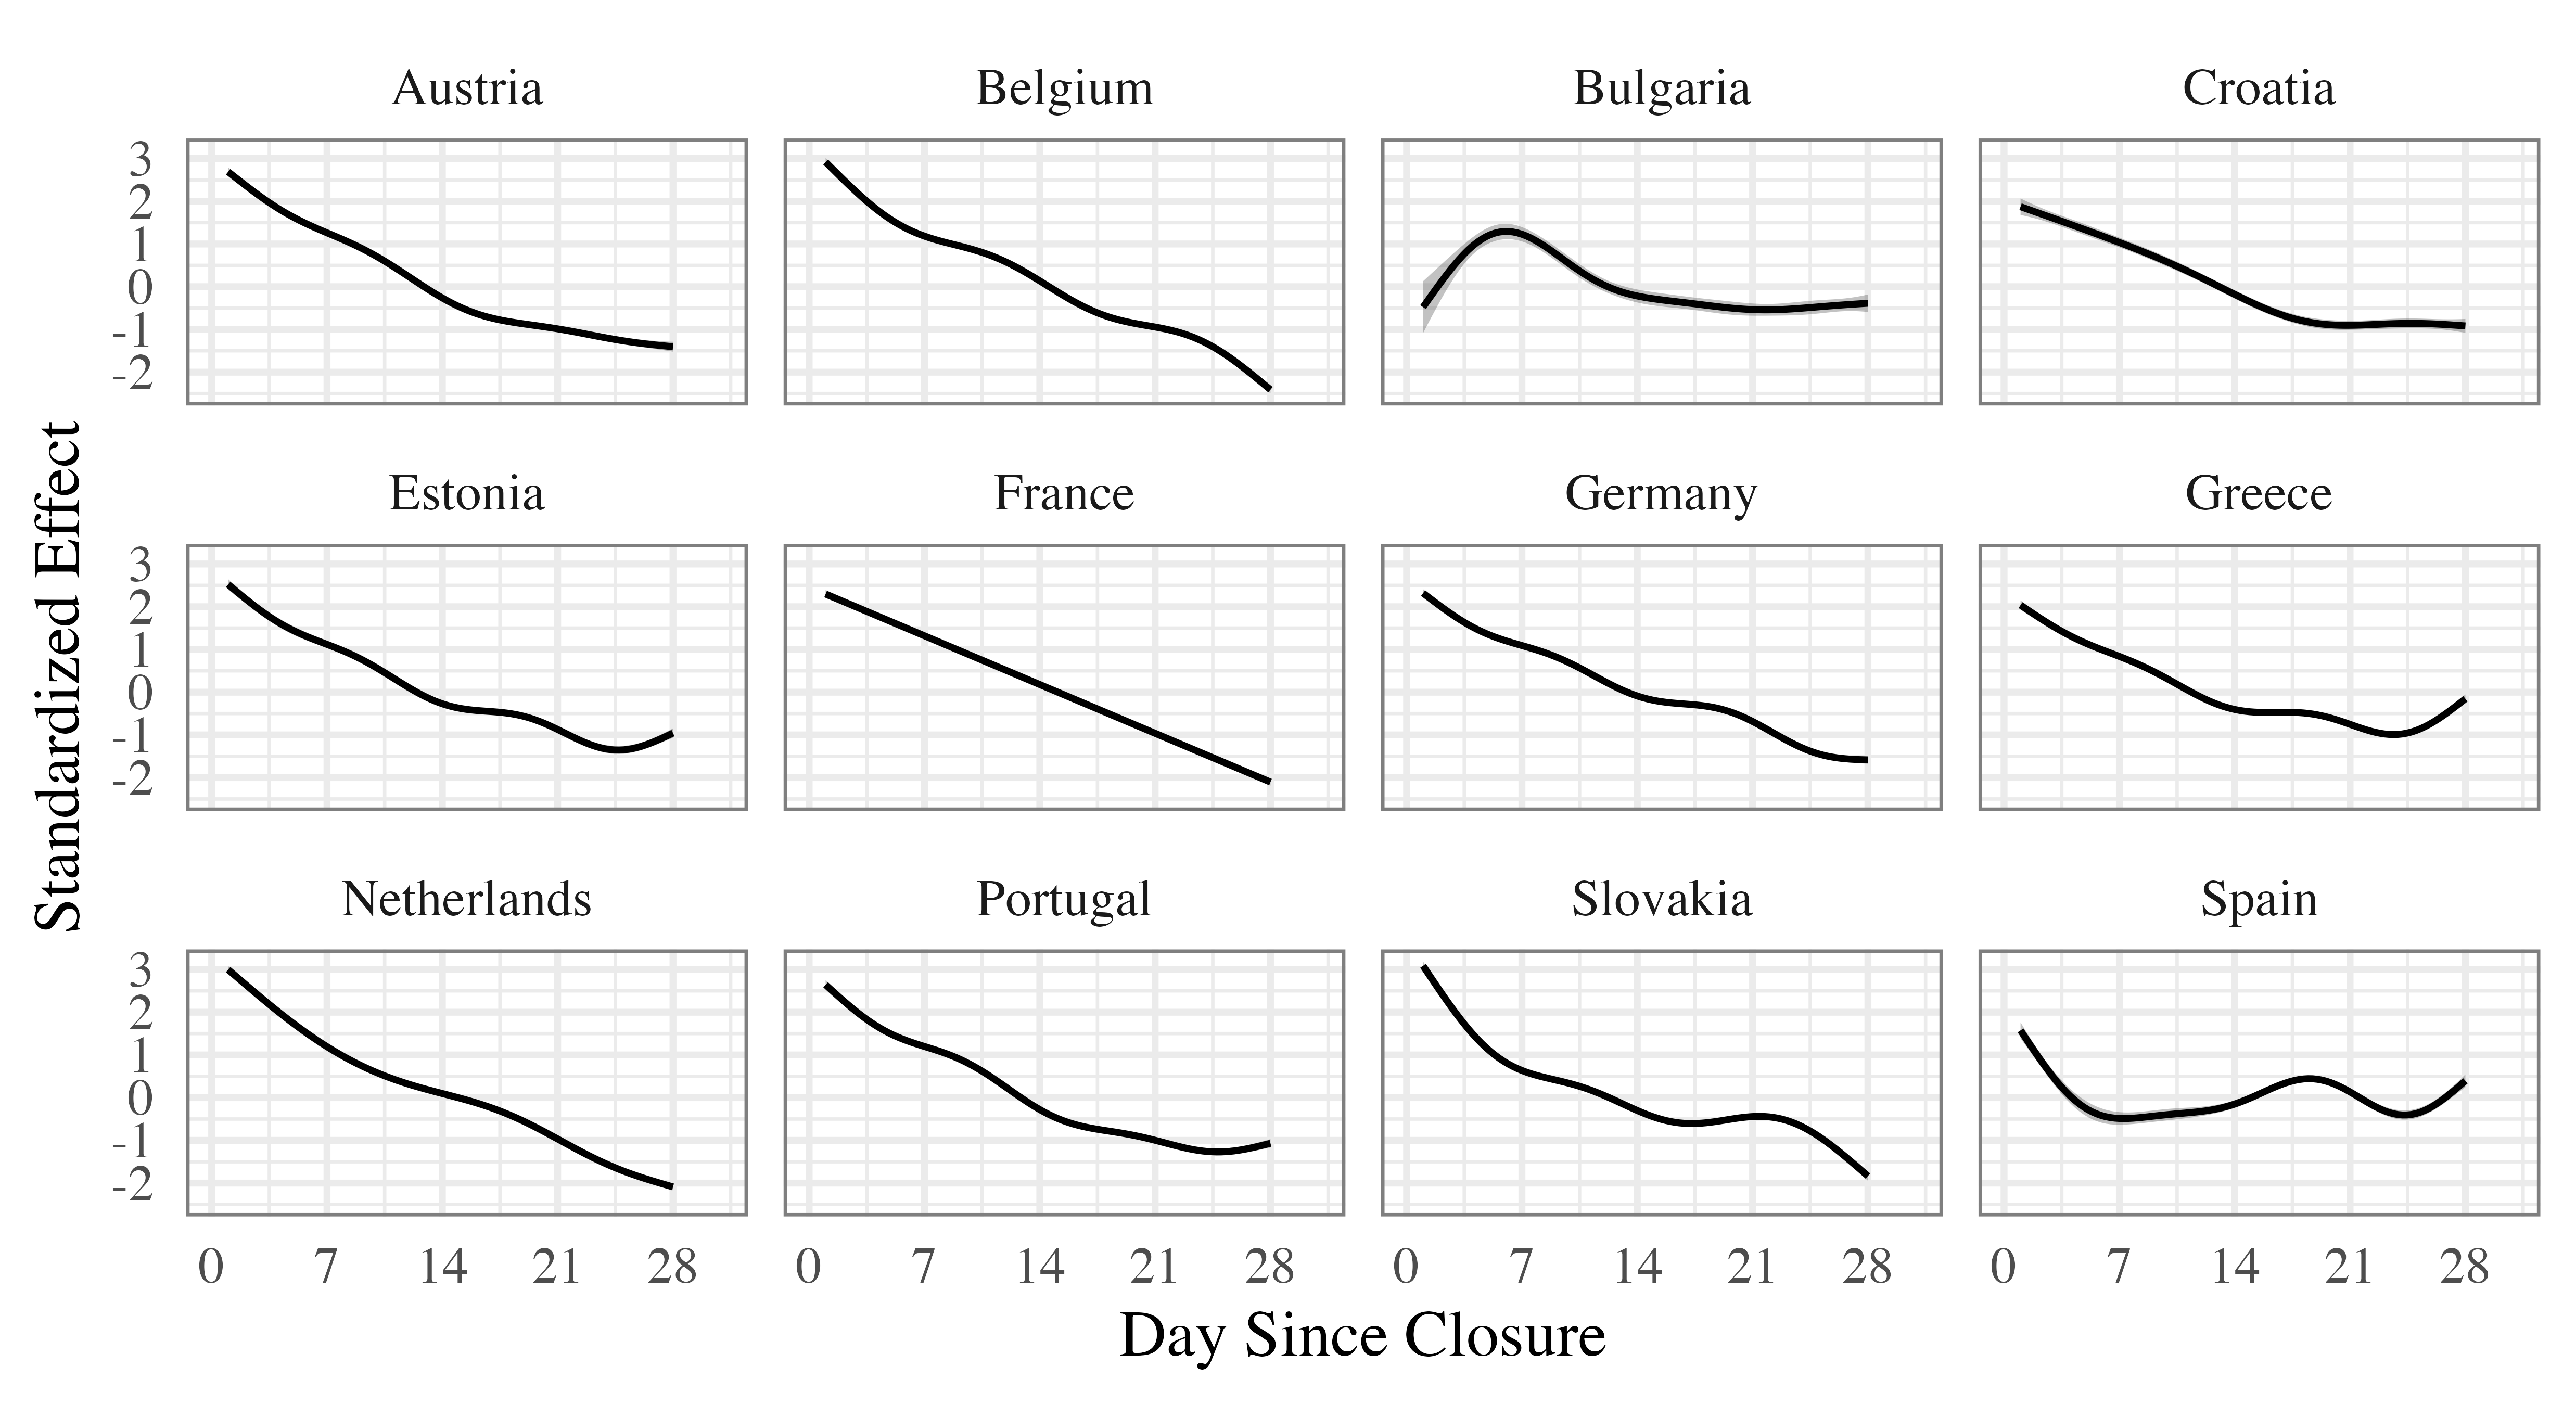
\includegraphics[keepaspectratio]{manuscript_files/figure-pdf/fig-country-1.png}}

}

\caption{\label{fig-country}Standardized effect of the smooth term in
Generalized Additive Model by country. Standardized effects are reported
to compare the shape of the curve between countries.}

\end{figure}%

While the general patterns described above were evident in the
aggregated analysis, country-specific smooths indicated some national
variations in the timing and magnitude of these age-specific effects,
although the paradoxical increase in the 5-14 age cohorts was observed
in a majority of countries.

\begin{figure}[h]

\centering{

\pandocbounded{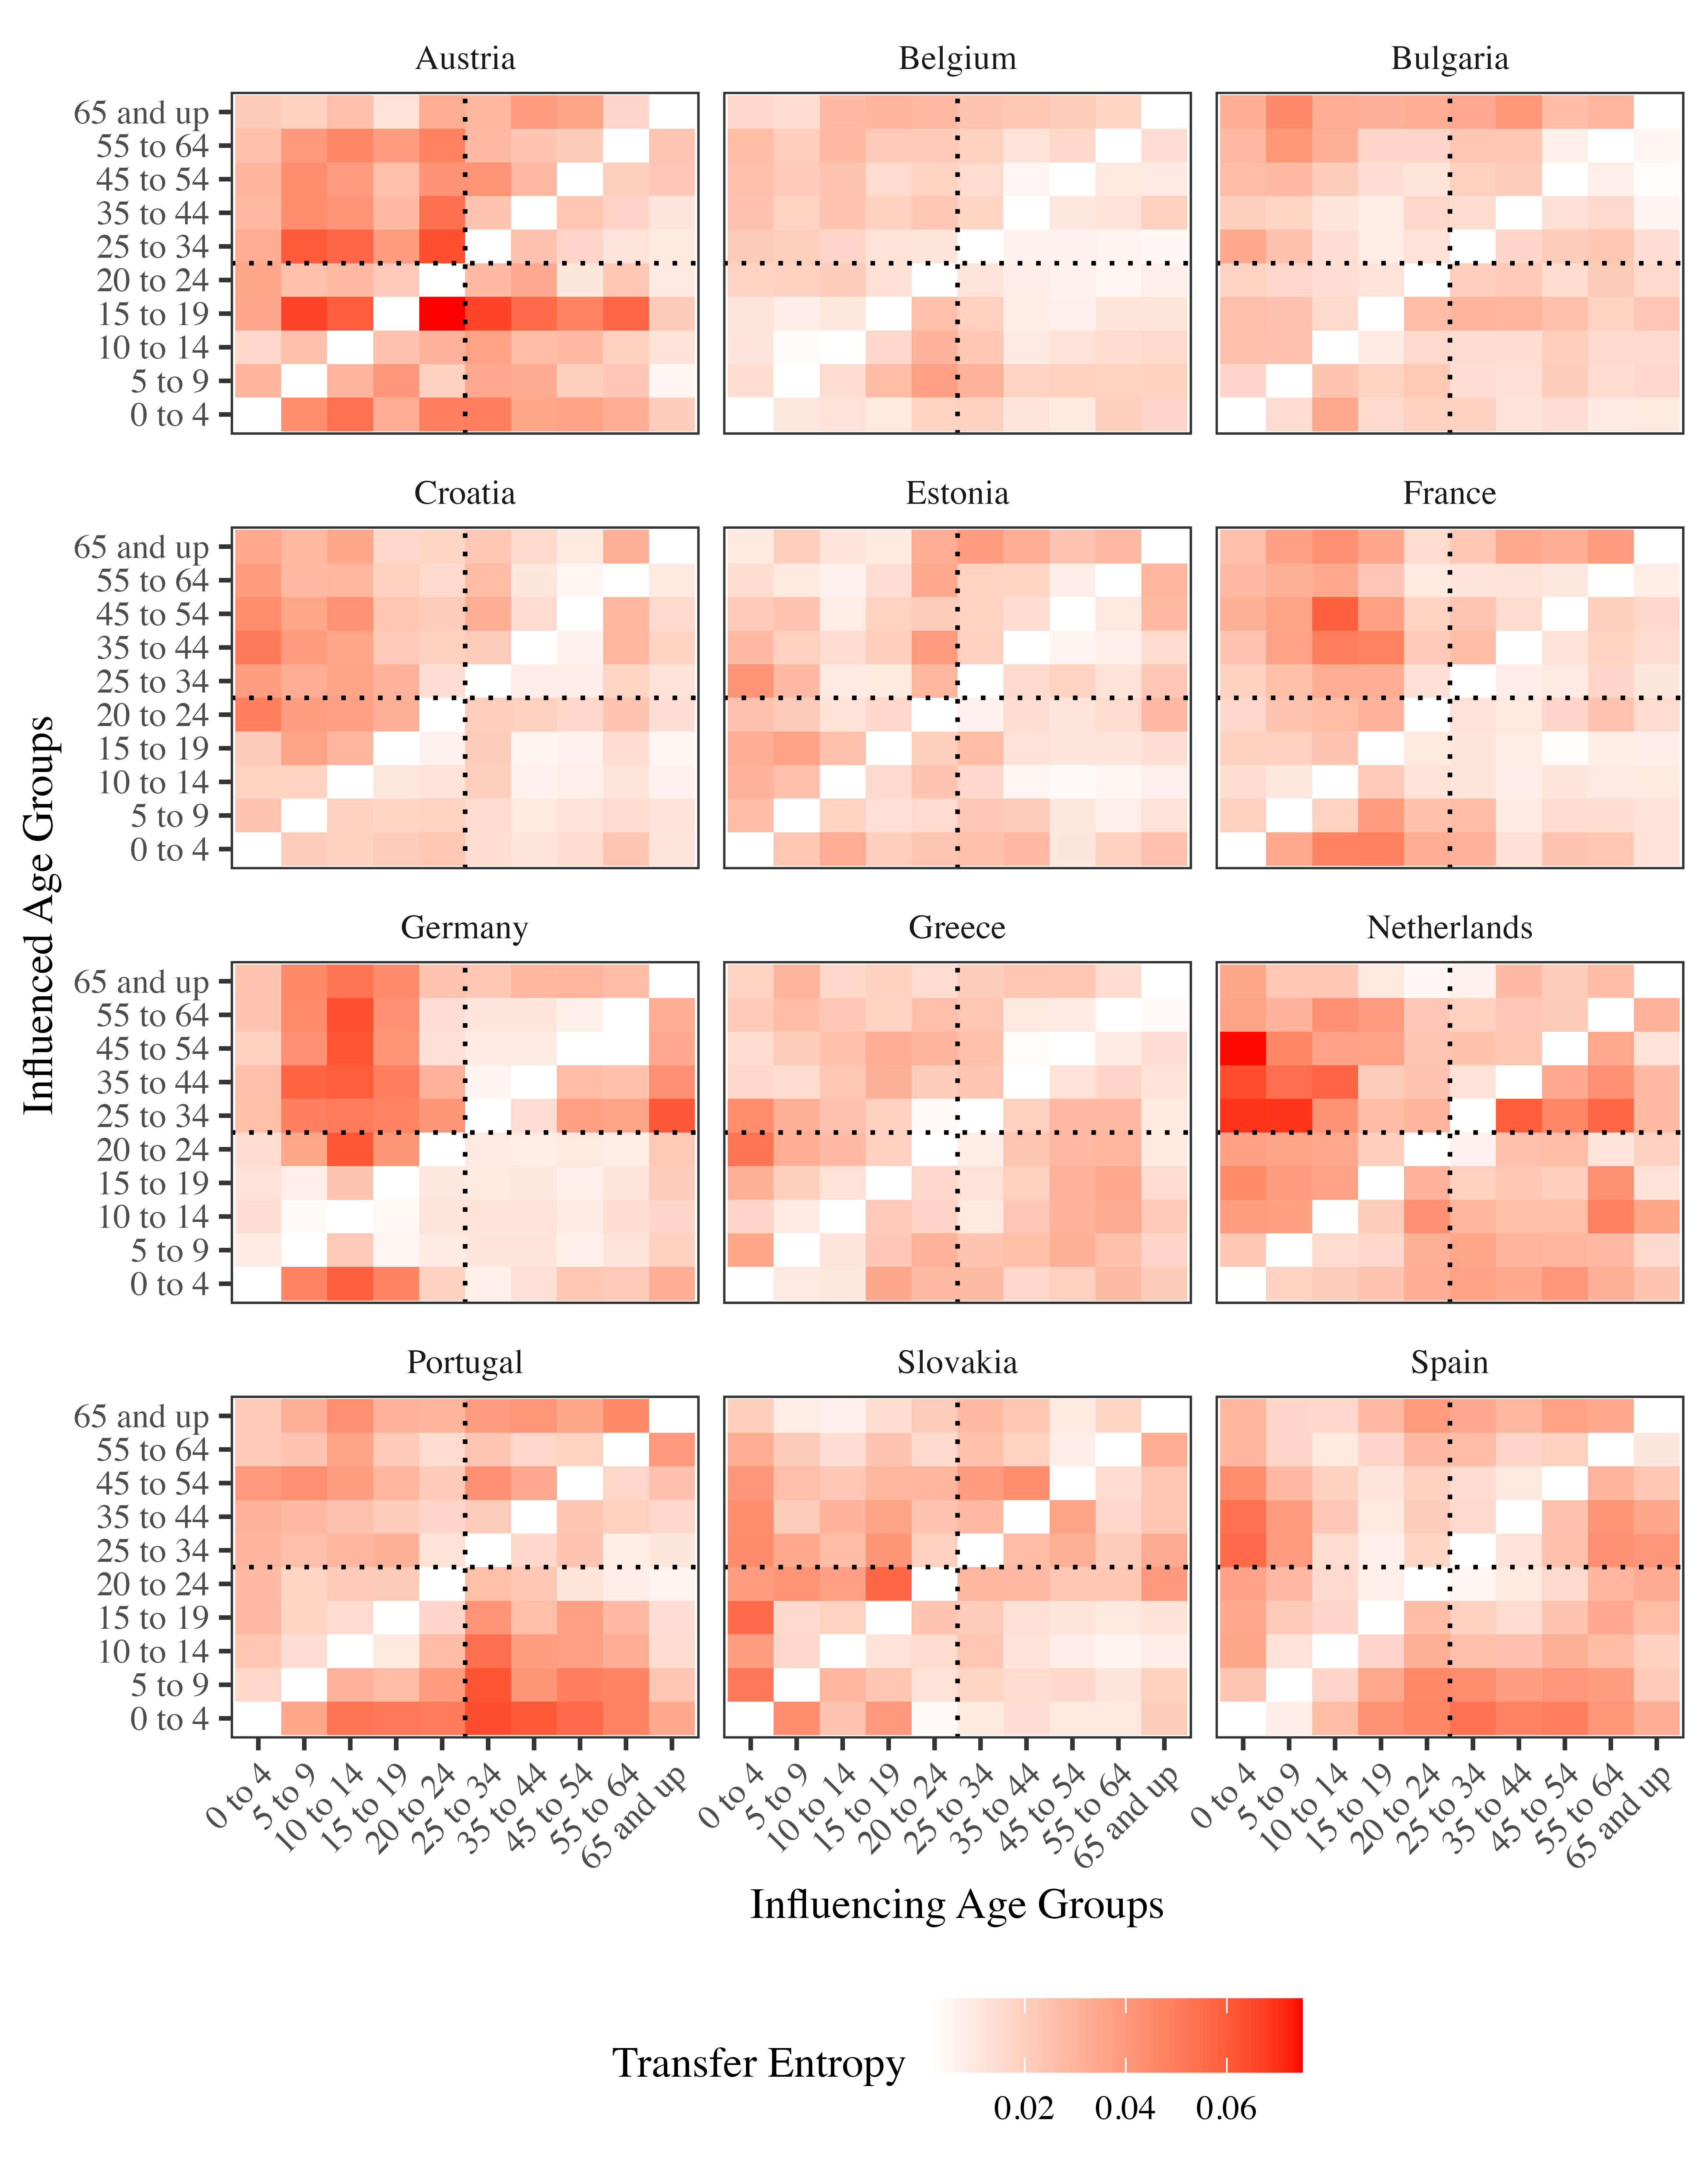
\includegraphics[keepaspectratio]{manuscript_files/figure-pdf/fig-te-1.png}}

}

\caption{\label{fig-te}Matrix of Transfer Entropy coefficients according
to every age group combination for each of the selected European
country. Age groups on the x-axis are influencing the age groups on the
y-axis (\(ag\,x \rightarrow\,ag\,y\)). The significance of each Transfer
Entropy coefficient is provided in Appendix 2.}

\end{figure}%

Considering all countries, the analysis of age groups reveals distinct
patterns (Figure~\ref{fig-te}). For the 0 to 4 age group, i.e., the
pre-school group, there was a downward trend during the initial three
weeks following school closure, followed by an increase during the
fourth week (\(\chi^2(5.96) = 410.48\), \(p < 0.001\)). A similar, but
more moderate, trend is observer for the age group ranging from 5 to 9
(\(\chi^2(5.95) = 878.29\), \(p < 0.001\)), where a decrease is observed
during the first two weeks, followed by an increase. while the trend for
the age group ranging from 10 to 14 is flat during the first two weeks,
a similar increase is shown at the beginning of the third week of school
closure (\(\chi^2(1) = 61.62\), \(p < 0.001\)). For age groups between
15 and 24, there is a notable surge immediately after school closure,
followed by a decrease after 14 days (15 to 19 age group:
\(\chi^2(5.97) = 7929.88\), \(p < 0.001\) and 20 to 24 age group:
\(\chi^2(4.98) = 18386.65\), \(p < 0.001\)). Thus, while the total case
number declined following school closures, among younger age groups only
the pre-school age group had a consistent reduction in cases, while for
other age groups, there was even an increase in cases following school
closures.

Given that school closures were not only aimed at reducing COVID-19
cases among school-going children but also age groups, it is important
to test the degree to which there was transmission across age groups,
which is done using transfer entropy analysis. Before this analysis is
carried out, an Augmented Dickey-Fuller has been applied to each age
group to ensure that the daily changes in COVID-19 cases are stationary
(see Appendix 1).

The results of the transfer entropy calculations between age groups for
each of the 12 selected European countries are reported in
Figure~\ref{fig-te}. The absence of symmetry between influencing age
groups (i.e., \(ag\,x\)) and influenced age groups (i.e., \(ag\,y\)) is
found. Indeed, the change in COVID-19 cases in some age groups is
influenced by other age groups, but they are not reciprocally
influencing these age groups. F@fig-te shows how different age cohorts
influence the COVID-19 case numbers of all age groups across countries.
The upper left quadrant indicates how younger age cohorts are
influencing older age cohorts, the bottom right quadrant indicates how
older age cohorts are influencing younger age cohorts, finally, the
lower left and upper right indicate how younger or older age cohorts are
influencing themselves. By analyzing these quadrants, it is possible to
identify similar patterns across multiple countries. Indeed, it appears
that Austria, Germany, and The Netherlands have significantly higher
\(T\) coefficients in the upper left quadrant of the matrix, which
indicates that the daily changes in COVID-19 cases number in younger
cohorts are predicting the daily changes in COVID-19 cases number in
older cohorts. Alternatively, it appears that Austria, the Netherlands,
Portugal, and Spain have significantly higher \(T\) coefficients in the
lower right quadrant of the matrix, which indicates that the daily
changes in COVID-19 cases number in older cohorts are predicting the
daily changes in COVID-19 cases number in younger cohorts.

\section{Discussion}\label{discussion}

Knowledge about the transmission of the virus significantly improved
over time as more studies have been published. While an early study
found that children did not play an important role in the transmission
of the virus \citep{li2020role}, more recent results give a more nuanced
position, stating that the spread of the virus in children is moderate.
It is now suggested that the impact of school openings on infection
rates was limited, with children and teachers more often contracting
infections through household or community contacts rather than within
schools \citep{soriano2023policies}. This study, using robust
statistical methods, considered the effect of school closures on
COVID-19 cases across age groups. While there are commonalities in the
evolution of COVID-19 cases across all European countries that were
included in our data, school closures exhibit distinct impacts on
different age groups. Notably, the analysis shows that the 0 to 4 age
group experiences a downward trend in COVID-19 cases during the initial
two weeks following school closure, followed by stabilization. In
contrast, age groups ranging from 5 to 14 exhibit a stable profile after
school closure. Additionally, age groups between 15 and 24 demonstrate a
notable surge immediately after school closure, followed by a decrease
after 14 days. Thus, the results do not support the hypothesis that
school closures were effective for group ages older than 5 years old.
One possibility is that school closures may lead to increased informal
social gatherings among children and teenagers outside of controlled
school environments, potentially facilitating virus transmission. It is
also possible that transmission within households intensified as
children spent more time at home. These results partially replicate
observations from \citet{alfano2022effects} while providing a clearer
picture of the structure of the effect of school closure.

The Transfer Entropy calculations between age groups for each of the 12
selected European countries reveal an absence of symmetry between
influencing age groups (\(X\)) and influenced age groups (\(Y\)). Some
age groups influence the COVID-19 case numbers of other age groups, but
there is no reciprocal influence. This finding suggests that changes in
COVID-19 cases in certain age groups can predict the changes in other
age groups but not vice versa, i.e., causality can be unidirectional.
These findings highlight the importance of considering intergenerational
interactions in designing effective control measures.

The entropy analysis revealed intriguing directional patterns of case
counts between age groups. In some countries, cases among younger
individuals appear predictive of cases among older individuals, while
the opposite pattern is observed elsewhere. These differences may
reflect country-specific variations in social mixing patterns,
healthcare responses, or policy measures. The absence of consistent
patterns in infections among adjacent age groups raises questions about
the mechanisms of transmission and suggests that factors beyond simple
proximity, such as behavioural differences or differing susceptibility,
may play a role. Future work should investigate these underlying
mechanisms to better understand age-based transmission dynamics.

Furthermore, the quadrant analysis reveals similar patterns across
multiple countries. Austria, Germany, and the Netherlands exhibit
significantly higher TE coefficients in the upper left quadrant,
indicating that changes in COVID-19 cases in younger cohorts predict the
changes in older cohorts. On the other hand, Austria, the Netherlands,
Portugal, and Spain show higher TE coefficients in the lower right
quadrant, indicating that changes in COVID-19 cases in older cohorts
predict the changes in younger cohorts. However, these differences may
also reflect country-specific variations in social mixing patterns,
healthcare responses, or policy measures. The absence of consistent
patterns in infections among adjacent age groups raises questions about
the mechanisms of transmission and suggests that factors beyond simple
proximity, such as behavioural differences or differing susceptibility,
may play a role.

This study, despite its methodological strengths, is subject to certain
limitations that warrant consideration. Foremost among these is the
inherent challenge of perfectly isolating the effect of school closures
from other simultaneously implemented and dynamically changing NPIs.
While we incorporated four composite NPI index derived from the Oxford
COVID-19 Government Response Tracker (OxCGRT) project to account for the
broader public health context, residual confounding from unmeasured
aspects of NPIs or behavioural changes may still persist. Our
sensitivity analyses showed consistent directional effects for school
closures even under varying overall NPI indexes provide some confidence,
but this remains an inherent complexity in observational studies of this
nature. Another consideration is the ecological design of the study,
which uses aggregated country-level data; this may mask important
sub-national variations and precludes inferences about individual-level
risk factors. In addition, the definition of ``closure'' which excluded
``partially open'' school statuses to simplify the intervention
definition, means the impact of such intermediate states was not
captured. Variations in testing strategies, case definitions, and
reporting practices across countries and over time could also have
influenced the observed case counts, despite efforts to use standardized
data sources. Lastly, this study predominantly covers periods before
widespread COVID-19 vaccination and the emergence of later variants such
as Omicron; the effects of school closures might differ under those
altered epidemiological conditions.

Future studies should look more closely at why the virus spread between
age groups as it did, and why TE patterns differed by country. This
could involve using information on people's behaviour or more detailed
data on other health rules. It would also be useful to study how
different virus types and vaccination levels change these effects.
Learning more about other influencing factors will help us better
understand the real impact of school closures.

\section{Conclusion}\label{conclusion}

This comprehensive analysis of COVID-19 school closures across 12
European nations reveals a complex and often counter-intuitive reality
that challenges prevailing assumptions about their universal efficacy,
particularly for children aged 5 and older. While national-level data
showed an overall decrease in cases during closures, our
age-disaggregated analysis using GAMs demonstrated that school-aged
children (5-14 years) and young adults (15-24 years) frequently
experienced periods of increased infections post-closure, a stark
contrast to the consistent reductions seen only in pre-schoolers.
Furthermore, Transfer Entropy analysis highlighted that the directional
influence of transmission between age groups was asymmetric and varied
by country, suggesting that the role of children in broader community
transmission during such periods is not uniform.

These findings underscore the critical importance of nuanced,
age-specific analysis in evaluating public health interventions and
caution against the broad application of measures like school closures
without robust evidence of their benefit across all targeted
demographics and a clear understanding of potential unintended
consequences \citep{alfano2020efficacy, molefi2021impact}. For future
pandemic preparedness, a more targeted, evidence-based approach is
essential, prioritising measures that minimise societal disruption while
effectively protecting public health across all age strata.

\section{Author statements}\label{author-statements}

\subsection{Ethical approval}\label{ethical-approval}

This study is a longitudinal analysis on available data; thus, it does
not require ethical approval.

\subsection{Funding}\label{funding}

None declared.

\subsection{Competing interests}\label{competing-interests}

None declared.

\subsection{Data Availability}\label{data-availability}

The data can be accessed from the COVerAGE-DB OSF repository
(https://osf.io/mpwjq/), from the Oxford Covid-19 Government Response
Tracker (OxCGRT) ``covid-policy-dataset'' GitHub repository
(https://github.com/OxCGRT/covid-policy-dataset), and from the UNESCO
servers
(https://en.unesco.org/file/unesco-data-school-closures-february-2020-june-2022csv-zip).
All preprocessing, analyses and code used to build the submitted paper
are available at https://github.com/damien-dupre/covid\_ts\_causality.

\section{References}\label{references}

\renewcommand{\bibsection}{}
\bibliography{bibliography.bib}

\end{document}
